
%***************************************************************************
%
% CreditCruncher - A portfolio credit risk valorator
% Copyright (C) 2004 Gerard Torrent
%
% This program is free software; you can redistribute it and/or
% modify it under the terms of the GNU General Public License
% as published by the Free Software Foundation; either version 2
% of the License.
%
% This program is distributed in the hope that it will be useful,
% but WITHOUT ANY WARRANTY; without even the implied warranty of
% MERCHANTABILITY or FITNESS FOR A PARTICULAR PURPOSE.  See the
% GNU General Public License for more details.
%
% You should have received a copy of the GNU General Public License
% along with this program; if not, write to the Free Software
% Foundation, Inc., 59 Temple Place - Suite 330, Boston, MA 02111-1307, USA.
%
%
% formulation.tex - TeX documentation file
% --------------------------------------------------------------------------
%
% 2005/01/22 - Gerard Torrent [gerard@fobos.generacio.com]
%   . initial release
%
%***************************************************************************

\chapter{Formulaci\'on del problema}
\label{sec:formulation}

\begin{center}
\framebox{
\begin{minipage}[c]{12.5cm}
Dada una cartera de cr\'editos a empresas de tama\~no mediano, deseamos 
valorar las posibles p\'erdidas debido a los impagos al cabo de un 
tiempo $T$.
\end{minipage}
}
\end{center}

A continuaci\'on se introducen los elementos y propiedades b\'asicas que 
constituyen el marco de trabajo.

%---------------------------------------------------------------------------

\section{Cartera de cr\'editos}

La estructura de la cartera de cr\'editos consiste en un conjunto de
clientes agrupados por sectores de actividad. Cada cliente tiene contratado 
un conjunto de productos de cr\'edito. Cada contrato puede estar 
cubierto por un n\'umero variable de garant\'ias o acuerdos.
Puede verse un esquema de la estructura en la figura \ref{portfolio}.

\begin{figure}[!hb]
\begin{center}
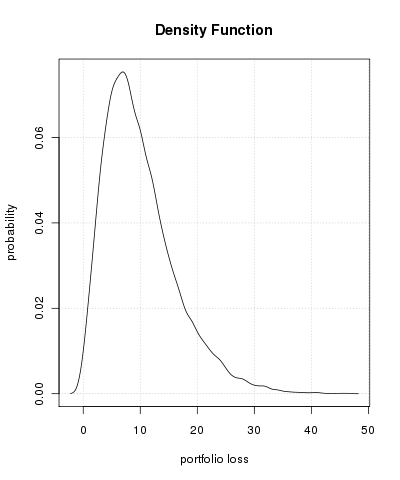
\includegraphics[width=6cm,angle=-90]{./images/portfolio.epsi}
\caption{Estructura de la cartera de cr\'editos}
\label{portfolio}
\end{center}
\end{figure}


\subsection{Ratings}

Un sistema de ratings es una medida de calidad crediticia usada para
valorar creditores. A cada creditor se le asigna una nota discreta (pe. AAA,
AA, A, BBB, BB, B, CCC, Default) en funci\'on de su calidad
crediticia. Los \'unicos ratings contemplados en este documento 
son los que tienen una relaci\'on estad\'istica directa y cuantificable 
con la probabilidad de impago del creditor. Ejemplos de este tipo de ratings 
son los publicados por Moody's Investor Service\footnote{http://www.moodys.com} 
o Standard \& Poors\footnote{http://www.standardandpoors.com}. 
\newline
\newline
La metodolog\'ia para la generaci\'on de un sistema de ratings queda fuera del
\'ambito de este documento. CreditCruncher presupone que cada empresa de la 
cartera tiene un rating inicial asignado.
\newline
\newline
El rating de cada empresa var\'ia a lo largo del tiempo en funci\'on de la 
calidad crediticia de cada instante (v\'ease figura \ref{ratingevol}). 
La evoluci\'on a lo largo del tiempo del rating de una empresa se 
formula a trav\'es de la matriz de transici\'on (v\'ease la secci\'on 
\ref{sec:mtransition}).
\begin{figure}[!hb]
\begin{center}
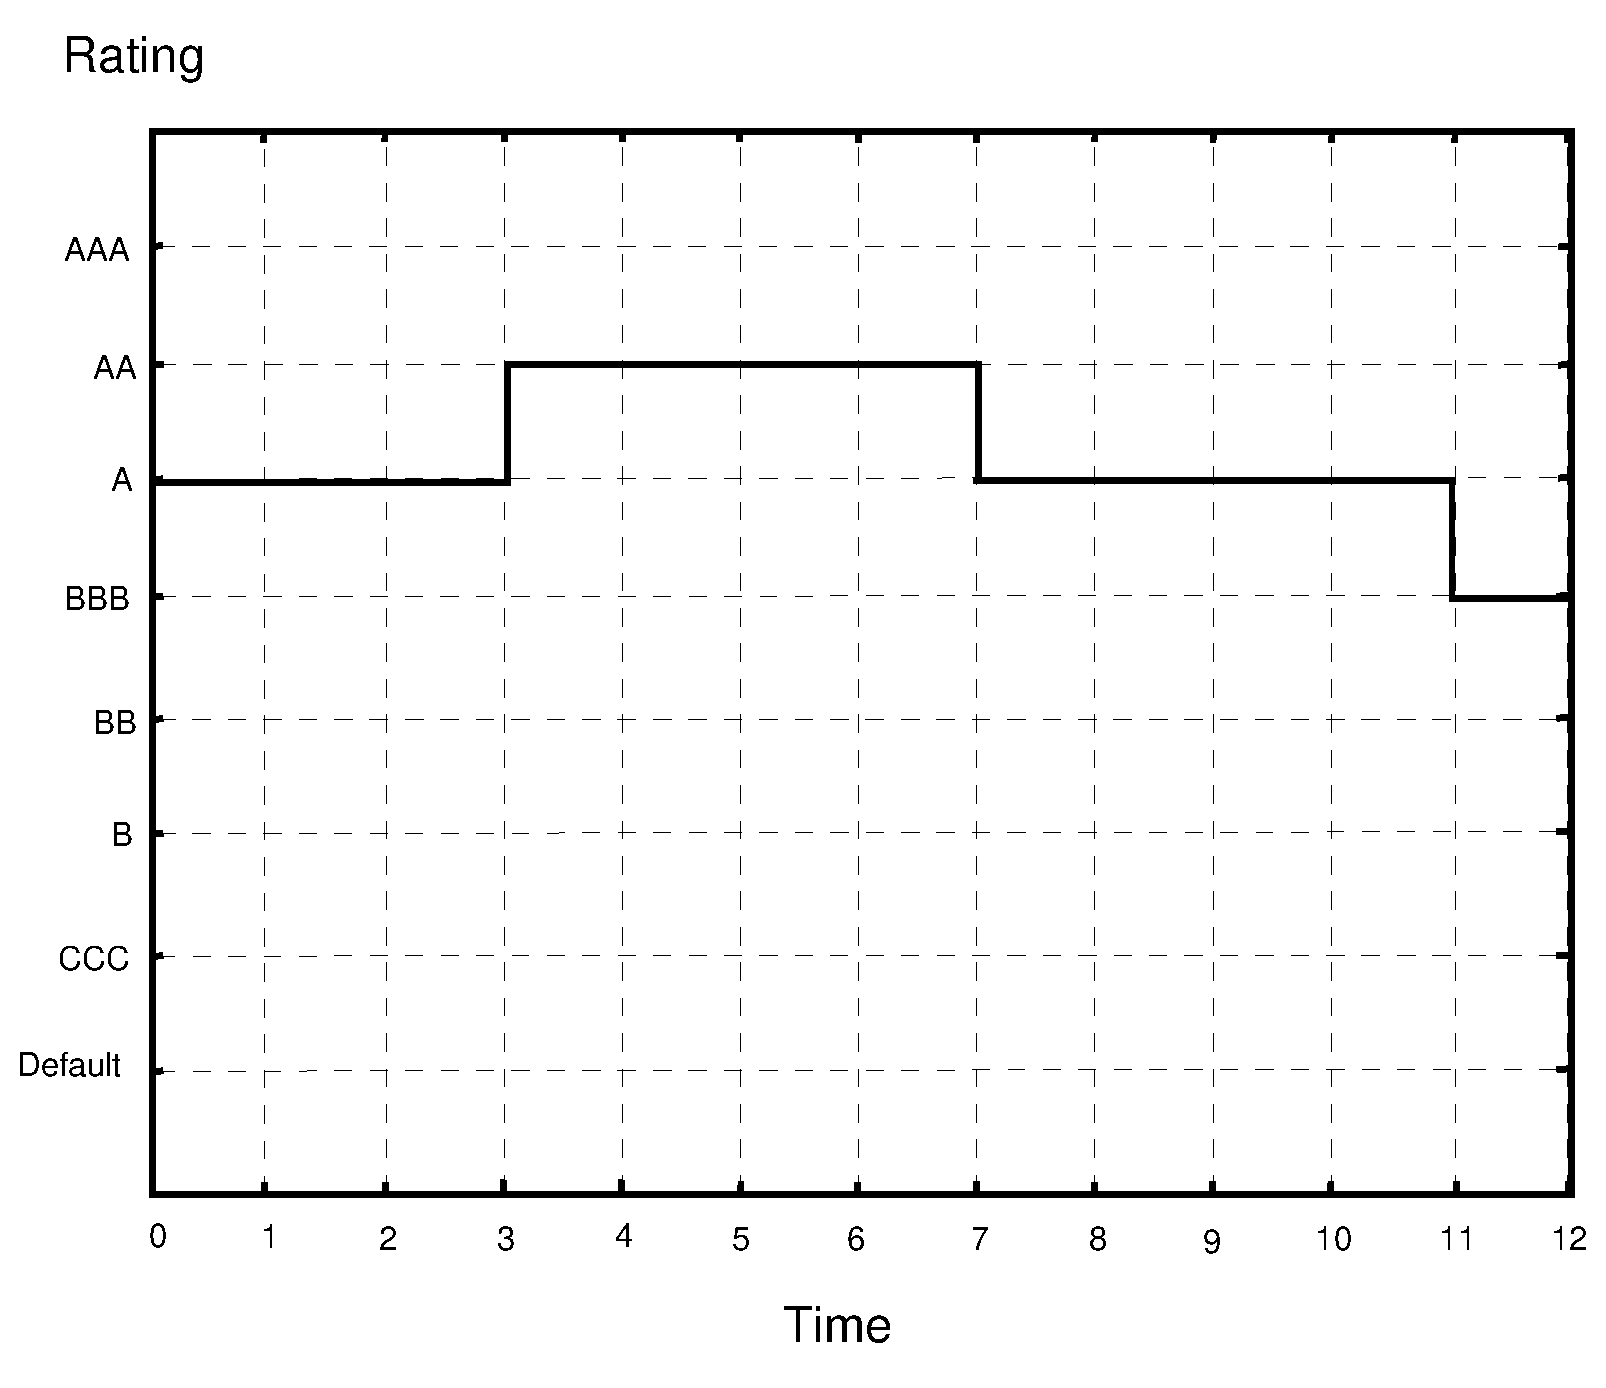
\includegraphics[height=6cm, angle=0]{./images/ratingevol.eps}
\caption{Evoluci\'on del rating a lo largo del tiempo}
\label{ratingevol}
\end{center}
\end{figure}
\paragraph{Notaci\'on.} El sistema de ratings usado en este documento se 
compone de $n$ notas, $r_1$, $r_2$, $\cdots$, $r_n$, donde $r_1$ es la
mejor nota (probabilidad de fallido mas baja), $r_2$ es la segunda mejor nota, 
etc. $r_n$ corresponde al rating $Default$.

\paragraph{Notaci\'on.} $P(r_i \to r_j;t) =$ probabilidad de pasar de un 
rating inicial $r_i$ a un rating $r_j$ en un tiempo $t$.


\subsection{Sectores}

La correlaci\'on de fallidos entre clientes es uno de los conceptos que
a\~naden complejidad de la valoraci\'on del riesgo de cr\'edito. No es lo
mismo tener una cartera de cr\'editos donde los clientes hacen fallido 
de forma independiente que una cartera donde los fallidos se encuentran 
correlacionados. En el primer caso, al cabo de un a\~no tendremos un 
conjunto limitado de fallidos. En el segundo caso, al cabo de un a\~no la 
mayoria de clientes habr\'an hecho fallido o casi ning\'un cliente habr\'a
hecho fallido. V\'ease el ejemplo \emph{Impacto de la correlaci\'on intrasectorial}.
\newline
\newline
Al no poder asignar una correlaci\'on de fallido cliente a cliente, se recurre
a la agrupaci\'on de estos en sectores. Se considera que la cartera de 
cr\'editos dispone de un conjunto de sectores donde los componentes de cada 
sector muestran una evoluci\'on crediticia similar (v\'ease figura \ref{sectors}). 
O sea, que la mejora o empeoramiento de la calidad crediticia (rating) afecta 
de forma com\'un a los componentes del sector. En general se identifican 
estos sectores con los sectores industriales. 

\begin{figure}[!hb]
\begin{center}
\includegraphics[height=6cm, angle=0]{./images/sectors.eps}
\caption{Sectores de actividad}
\label{sectors}
\end{center}
\end{figure}
Se considera que cada cliente pertenece a un \'unico sector y permanece en 
el a lo largo del tiempo. La relaci\'on entre sectores se formula a trav\'es 
de la matriz de correlaci\'on sectorial (v\'ease la secci\'on \ref{sec:mcorrel}).
\paragraph{Notaci\'on.} En este documento se considera que existen $m$ 
sectores, y nos referiremos a ellos como $s_1$, $s_2$, $\cdots$, $s_m$.

\subsection{Activos}

Cada cliente tiene contratado un conjunto de activos con riesgo de cr\'edito.
Un activo se caracteriza por los siguientes elementos:

\paragraph{Cashflow.} Entregas y devoluciones de dinero a lo largo del tiempo. 
Incluye las posibles amortizaciones, primas, cupones, comisiones, costes, etc. 
Usaremos el cashflow para calcular el valor, o precio, de un activo en el 
instante $t$.

\paragraph{Exposici\'on.} Importe de la p\'erdida en caso de fallido. Cada 
producto tiene un perfil de exposici\'on caracter\'istico.

\paragraph{Recuperaci\'on.} Importe que se estima que ser\'a recuperado en 
caso de fallido. Normalmente es una parte de la exposici\'on.


\begin{figure}[!hb]
\begin{center}
\includegraphics[height=10cm, angle=-90]{./images/mortgage.ps}
\caption{Perfil de un Pr\'estamo Hipotecario}
\label{mortgage}
\end{center}
\end{figure}


\begin{figure}[!hb]
\begin{center}
\includegraphics[height=10cm, angle=-90]{./images/endorsement.ps}
\caption{Perfil de un Aval financiero}
\label{endorsement}
\end{center}
\end{figure}

\begin{figure}[!hb]
\begin{center}
\includegraphics[height=10cm, angle=-90]{./images/bond.ps}
\caption{Perfil de un Bono}
\label{bond}
\end{center}
\end{figure}

Exposici\'on, Severidad

%---------------------------------------------------------------------------

\section{Matriz de transici\'on}
\label{sec:mtransition}

\subsection{Definici\'on} La matriz de transici\'on nos proporciona la probabilidad 
que un cliente con rating inicial $r_i$ pase a tener, al cabo de un tiempo $T$, 
rating $r_j$. La denotamos de la forma siguiente:

\begin{displaymath}
M_T = \left(
\begin{array}{ccc}
m_{1,1} & \dots  & m_{1,n} \cr
\vdots & \ddots & \vdots \cr
m_{n,1} & \dots  & m_{n,n} 
\end{array}
\right)
\qquad
m_{i,j} = P(r_i \to r_j;T)
\end{displaymath}

\noindent donde cada elemento de la matrix, $m_{i,j}$ corresponde a la 
probabilidad de que un cliente con rating $r_i$ pase a tener, al cabo de $T$ 
tiempo, rating $r_j$.

\subsection{Ejemplo} Matriz de transici\'on anual ($T=1$ a\~no) extraida del 
documento \emph{CreditMetrics - Technical Document} \cite{CreditMetrics:Tech_Doc}. 
Las probabilidades est\'an expresadas en tanto por ciento.
\\
\begin{center}
\begin{tabular}[]{l|rrrrrrrr}
        &      AAA &       AA &        A &      BBB &       BB &        B &      CCC &  Default \cr
\hline
AAA     &  $90.81$ &   $8.33$ &   $0.68$ &   $0.06$ &   $0.12$ &   $0.00$ &   $0.00$ &   $0.00$ \cr
 AA     &   $0.70$ &  $90.65$ &   $7.79$ &   $0.64$ &   $0.06$ &   $0.14$ &   $0.02$ &   $0.00$ \cr
  A     &   $0.09$ &   $2.27$ &  $91.05$ &   $5.52$ &   $0.74$ &   $0.26$ &   $0.01$ &   $0.06$ \cr
BBB     &   $0.02$ &   $0.33$ &   $5.95$ &  $86.93$ &   $5.30$ &   $1.17$ &   $0.12$ &   $0.18$ \cr
 BB     &   $0.03$ &   $0.14$ &   $0.67$ &   $7.73$ &  $80.53$ &   $8.84$ &   $1.00$ &   $1.06$ \cr
  B     &   $0.00$ &   $0.11$ &   $0.24$ &   $0.43$ &   $6.48$ &  $83.46$ &   $4.07$ &   $5.20$ \cr
CCC     &   $0.22$ &   $0.00$ &   $0.22$ &   $1.30$ &   $2.38$ &  $11.24$ &  $64.86$ &  $19.79$ \cr
Default &   $0.00$ &   $0.00$ &   $0.00$ &   $0.00$ &   $0.00$ &   $0.00$ &   $0.00$ & $100.00$
\end{tabular}
\end{center}
En particular, la probabilidad que un cliente con rating $AA$ pase a tener 
rating $B$ al cabo de un a\~no es del $0.14\%$.

\subsection{Propiedades}

\paragraph{Propiedad 1.}
El valor de los elementos de la matriz de transici\'on se encuentran entre $0$ 
y $1$ debido a que los elementos de la matriz son probabilidades.

\begin{displaymath}
0 \leq m_{i,j} \leq 1 \quad \forall i,j
\end{displaymath}

\paragraph{Propiedad 2.}
La suma de los elementos de cualquier fila de la matriz de transici\'on suman $1$.
De esta forma se  est\'a imponiendo que el conjunto de ratings finales solo puede 
ser el de los ratings contemplados en la matriz.

\begin{displaymath}
\sum_{j=1}^{n} m_{i,j} = 1 \quad \forall i
\end{displaymath}

\paragraph{Propiedad 3.}
Los elementos de la fila correspondiente al rating $Default$ ($r_n$), son todos 
$0$, excepto el elemento de la columna que corresponde al rating $Default$, 
$m_{n,n}$, que vale $1$. Esta condici\'on indica que cuando se llega al estado 
de fallido no es posible salir de este estado.

\begin{displaymath}
\begin{array}{ll}
m_{n,j} = 0        & \quad \forall j \neq n \cr
m_{n,n} = 1
\end{array}
\end{displaymath}


\subsection{Cambio de periodo}

Deseamos obtener la matriz de transici\'on para periodos distintos (m\'ultiplos o 
fraccionarios) del periodo proporcionado, $T$. Esto nos permitir\'a determinar la 
probabilidad que un cliente con rating inicial $r_i$ tenga rating $r_j$ al cabo 
de $k \cdot T$ tiempo o al cabo de $K/t$ tiempo.

\paragraph{Ejemplo.} Calculemos la probabilidad de pasar de rating $AA$ a
rating $B$ en un plazo de dos a\~nos disponiendo de la matriz de transici\'on anual.

\begin{displaymath}
\begin{array}{llll}
P(AA \to B;2) = & P(AA \to AAA;1)    & \cdot P(AAA \to B;1)      & + \cr
                & P(AA \to AA;1)      & \cdot P(AA \to B;1)      & + \cr
                & P(AA \to A;1)       & \cdot P(A \to B;1)       & + \cr
                & P(AA \to BBB;1)     & \cdot P(BBB \to B;1)     & + \cr
                & P(AA \to BB;1)      & \cdot P(BB \to B;1)      & + \cr
                & P(AA \to B;1)       & \cdot P(B \to B;1)       & + \cr
                & P(AA \to CCC;1)     & \cdot P(CCC \to B;1)     & + \cr
                & P(AA \to Default;1) & \cdot P(Default \to B;1) &
\end{array}
\end{displaymath}

\paragraph{Proposici\'on.} Sean $M_{T_1}$ y $M_{T_2}$ las matrices de transici\'on
para los periodos $T_1$ y $T_2$. Entonces, la matriz de transici\'on para el
periodo $T_1+T_2$ es:
\begin{displaymath}
M_{T_1+T_2} = M_{T_1} \cdot M_{T_2}
\end{displaymath}

\paragraph{Corolario.} Sean $M_{T}$ la matriz de transici\'on para el periodo 
$T$ y $k \in \mathrm{N}$. Entonces:
\begin{displaymath}
M_{k \cdot T} = M_{T}^k
\end{displaymath}
\begin{displaymath}
M_{\frac{T}{k}} = \sqrt[k]{M_{T}}
\end{displaymath}


\subsection{Tasa de morosidad anticipada}


%---------------------------------------------------------------------------

\section{Matriz de correlaci\'on sectorial}
\label{sec:mcorrel}

\subsection{Definici\'on} blablabla

\subsection{Ejemplo} blablabla

\subsection{Propiedades} blablabla
%---------------------------------------------------------------------------

\section{Value At Risk (VAR)}

\begin{figure}[!hb]
\begin{center}
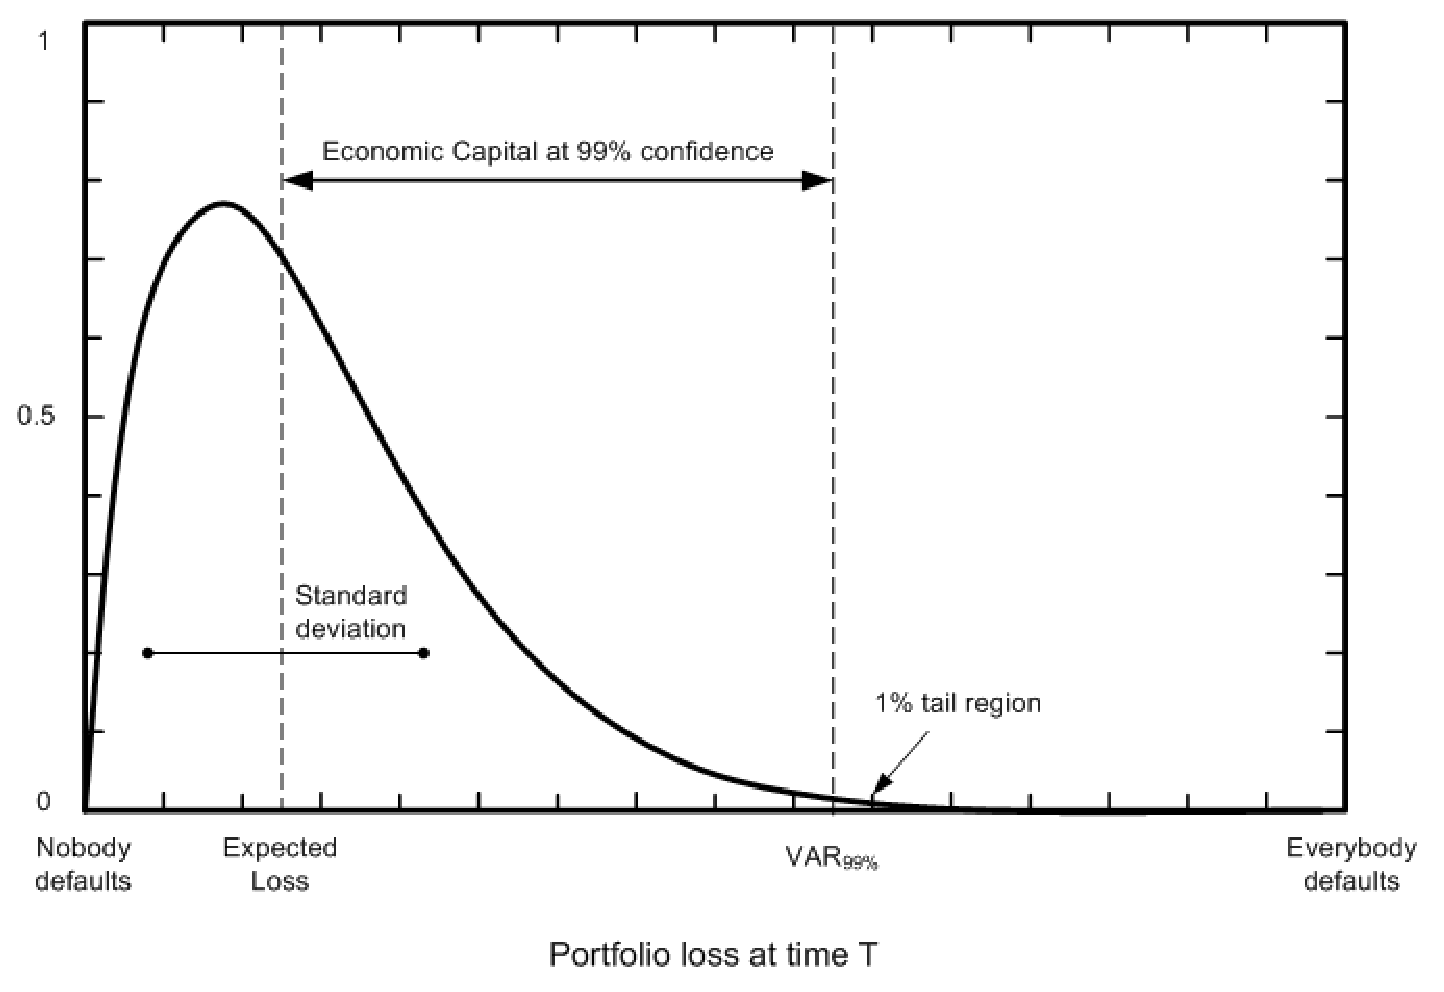
\includegraphics[height=7cm, angle=0]{./images/creditvar.eps}
\caption{Distribuci\'on del valor de la cartera y c\'alculo del VAR}
\label{creditvar}
\end{center}
\end{figure}
